\documentclass[12pt]{article}
\usepackage{amsmath}
\usepackage{graphicx}
\usepackage{hyperref}
\usepackage{listings}
\usepackage{color}
\usepackage{pythonhighlight}
\usepackage{enumerate}

\title{Operating System Course Report - First Half of the Semester}
\author{A class}
\date{\today}

\begin{document}

\maketitle
\newpage

\tableofcontents
\newpage

\section{Introduction}
This report summarizes the topics covered during the first half of the Operating System course. It includes theoretical concepts, practical implementations, and assignments. The course focuses on the fundamentals of operating systems, including system architecture, process management, CPU scheduling, and deadlock handling.

\section{Course Overview}
\subsection{Objectives}
The main objectives of this course are:
\begin{itemize}
    \item To understand the basic components and architecture of a computer system.
    \item To learn process management, scheduling, and inter-process communication.
    \item To explore file systems, input/output management, and virtualization.
    \item To study the prevention and handling of deadlocks in operating systems.
\end{itemize}

\subsection{Course Structure}
The course is divided into two halves. This report focuses on the first half, which covers:
\begin{itemize}
    \item Basic Concepts and Components of Computer Systems
    \item System Performance and Metrics
    \item System Architecture of Computer Systems
    \item Process Description and Control
    \item Scheduling Algorithms
    \item Process Creation and Termination
    \item Introduction to Threads
    \item File Systems
    \item Input and Output Management
    \item Deadlock Introduction and Prevention
    \item User Interface Management
    \item Virtualization in Operating Systems
\end{itemize}

\section{Topics Covered}

\subsection{Basic Concepts and Components of Computer Systems}
This section explains the fundamental components that make up a computer system, including the CPU, memory, storage, and input/output devices.
\subsubsection{Jenis-Jenis Komputer}
\subsubsection{Hardware}
\subsubsection{Software}
    \par
    \hspace{0.61cm}\textit{Software} adalah sekumpulan instruksi kode dan data-data tertentu yang berfungsi untuk menjalankan sebuah program atau perintah yang ada didalam komputer. Program yang akan dijalankan tentunya akan memerlukan sebuah \textit{hardware} atau perangkat keras yang dimiliki agar perangkat lunak berjalan optimal.\cite{IDCloudHost}

    Dalam pembuatannya, \textit{software} dibuat oleh seorang programmer atau pengembang perangkat lunak. Perangkat lunak ini dibuat dengan menggunakan bahasa pemrograman tertentu yang kemudian akan diubah menjadi kode mesin agar dapat dijalankan oleh komputer.\cite{JagoanHosting}

    \textit{Software} dirancang untuk memfasilitaskan pekerjaan manusia. Contoh-nya seperti menghitung, membuat dokumen, mengedit gambar, dan sebagainya. Selain itu, dengan \textit{software} kamu juga bisa melakukan pengeditan video, pembuatan desain, permainan \textit{game}, dan masih banyak lagi.\cite{JagoanHosting}

    \begin{itemize}
        
        \item \textbf{Ciri-ciri \textit{Software}} 
        \par
        Namun meski secara jelas \textit{software} memiliki kegunaan dalam menjalankan sebuah perintah atau fitur tertentu dalam komputer, \textit{software} juga memiliki ciri spesifik. Berikut beberapa ciri-ciri jika program tersebut adalah sebuah \textit{software} :
        \begin{itemize}
            \item Penunjang \textit{hardware}
            \par
            \textit{Software} bertanggung jawab untuk mengelola perangkat keras pada komputer. Perangkat keras juga terkadang membutuhkan pemrograman yang dihasilkan dari perangkat lunak untuk bekerja secara sempurna. Komputer atau gadget tentunya akan berfungsi dengan baik jika pemrograman dilakukan sesuai dengan fungsi dan perintah.\cite{IDCloudHost}\cite{JagoanHosting}
            \item Memiliki sumber terbuka atau bersifat komersil
            \par
            Dalam menginstal sebuah perangkat lunak terkadang developer dapat dengan mudah mengunduhnya secara gratis. Hal ini disebabkan memang ada beberapa perusahaan yang dengan sengaja menerapkan \textit{Open source} pada \textit{software} mereka. Namun juga ada beberapa pengembang yang menerapkan sistem berbayar pada \textit{software} yang dikembangkannya.\cite{IDCloudHost}
            \item Membutuhkan \textit{File Installer}
            \par
            Dalam melakukan pemasangan sebuah \textit{software} kedalam sebuah komputer tentunya akan membutuhkan yang dinamakan dengan \textit{File Installer}.\cite{IDCloudHost}
            \item Rentan Terhadap Virus
            \par
            Baik sebelum mengunduh maupun setelah mengunduh \textit{software}, komputer Anda akan jauh lebih rentan terkena virus saat menjalankannya. Hal tersebut juga tidak dapat dipungkiri perangkat lunak yang akan digunakan mungkin sudah terdapat virus di-dalamnya.\cite{JagoanHosting}
        \end{itemize}

        \item \textbf{Jenis-Jenis \textit{Software}}
        \par
        Secara umum, perangkat lunak terbagi menjadi 2, yaitu :
        \begin{enumerate}
            \item \textit{Software System}
            \par
            \textit{Software System} Merupakan \textit{software} yang paling dasar dalam sebuah komputer, bertugas untuk mengelola semua \textit{hardware} komputer dan menyediakan layanan umum bagi \textit{software} lain.\cite{Gramedia} Contoh \textit{Software System} yang paling umum, yaitu :
            \begin{itemize}
                \item Sistem Operasi (\textit{Operating System/OS})
                \par
                \textit{Software} yang bertugas untuk mengelola semua sumber daya komputer, seperti \textit{hardware}, \textit{software}, dan data. Sistem Operasi juga bertanggung jawab untuk menjalankan program-program aplikasi dan memberikan antarmuka pengguna agar pengguna dapat berinteraksi dengan komputer. Contohnya, \textit{Windows, macOS, Linux,} dll.
                \item \textit{Driver}
                \par 
                \textit{Software} yang bertugas untuk menghubungkan perangkat ke-ras dengan sistem operasi. 
                \textit{Driver} memungkinkan sistem operasi untuk mengenali dan berkomunikasi dengan perangkat keras, seperti \textit{printer}, \textit{scanner}, dan kartu grafis.
                \item \textit{Utility Software}
                \par
                \textit{Software} yang dirancang untuk membantu pengguna dalam mengelola, mengoptimalkan, dan memperbaiki sistem komputer. \textit{Utility Software} dapat digunakan untuk membersihkan \textit{file} sampah, mempercepat kinerja komputer, dan memperbaiki kesalahan sistem. Contohnya, \textit{antivirus, disk cleaner,} dan \textit{system optimizer}.
            \end{itemize} 
            \item \textit{Software} Aplikasi
            \par
            \textit{Software} Aplikasi merupakan \textit{software} yang sudah banyak digunakan di suatu bidang tertentu. Jenis perangkat lunak ini dibuat untuk mengerjakan suatu fungsi atau perintah khusus yang terdapat didalam komputer.\cite{Gramedia} Contoh \textit{Software} Aplikasi yang paling umum, yaitu :
            \begin{itemize}
                \item \textit{Software Productivity}
                \par
                \textit{Software} yang dirancang untuk membantu pengguna dalam menyelesaikan tugas sehari-hari, seperti membuat dokumen, mengelola data, dan membuat presentasi. Contohnya, \textit{Microsoft Office, Google Docs,} dan \textit{LibreOffice}.
                \item \textit{Software} Multimedia
                \par
                \textit{Software} yang dirancang untuk mengakses \textit{file} multimedia, seperti gambar, video, dan audio. \textit{Software} Multimedia dapat digunakan untuk melihat foto, menonton video, dan mendengarkan musik. Contohnya, \textit{Spotify, Photos} dan \textit{Media Player}.
                \item \textit{Software} Kreativitas
                \par
                \textit{Software} yang dirancang untuk membantu pengguna dalam membuat konten kreatif, seperti desain grafis, animasi, dan pengembangan web. Contohnya, \textit{Adobe Photoshop, Blender,} dan \textit{WordPress}.
                \item \textit{Software Game}
                \par
                \textit{Software} yang dirancang untuk memberikan hiburan kepada pengguna dalam bentuk permainan. \textit{Software} \textit{Game} dapat digunakan untuk bermain \textit{game} tunggal atau bermain \textit{game} online dengan pemain lain. Contohnya, \textit{Minecraft, Fortnite,} dan \textit{League of Legends}.
                \item \textit{Software} Web \textit{Browser}
                \par
                \textit{Software} yang dirancang untuk mengakses dan menjelajahi di internet. \textit{Software} Web \textit{Browser} dapat digunakan untuk mencari informasi, berbelanja \textit{online}, dan berkomunikasi dengan orang lain. Contohnya, \textit{Google Chrome, Mozilla Firefox,} dan \textit{Microsoft Edge}.
            \end{itemize}
        \end{enumerate}

        \item \textbf{Jenis Software Berdasarkan Distribusinya}
        \par
        \textit{Software} atau perangkat lunak juga memiliki beberapa pendistribusiannya. Diketahui ada 7 jenis \textit{software} yang memiliki klasifikasi fungsi dan pekerjaan yang berbeda.\cite{IDCloudHost}\cite{Gramedia} Berikut penjelasan mengenasi 7 tipenya:
        \begin{enumerate}
            \item \textbf{\textit{Adware}}
            \par
            \textit{Adware} secara khusus diciptakan untuk membagikan beberapa iklan secara luas kedalam komputer terutama ketika sedang berada didalam internet.  Jenis perangkat lunak ini juga bisa menghasilkan pendapatan melalui metode \textit{pay per click} (PPC).\cite{IDCloudHost}
            \item \textbf{\textit{Firmware}}
            \par
            Perangkat lunak ini berguna sebagai sistem operasi yang terdapat pada komputer khususnya pada bagian perangkat keras. Penyimpanan perangkat lunak ini bersifat hanya baca  sehingga tidak perlu lagi melakukan modifikasi maupun pengembangan lebih lanjut meskipun terjadi masalah pada fungsinya.\cite{IDCloudHost}
            \item \textbf{\textit{Freeware}}
            \par
            Merupakan salah satu jenis \textit{software} yang tidak memiliki batas waktu tertentu. Akan tetapi, kebanyakan \textit{software} jenis ini memiliki fitur yang tidak begitu lengkap sehingga penggunaannya pun kurang maksimal.\cite{Gramedia}
            \item \textbf{\textit{Malware}}
            \par
            Merupakan salah satu jenis dari \textit{software} yang dianggap berbahaya dan bisa merusak apabila disalahgunakan penggunaannya. Program perangkat lunak ini secara spesifik digunakan untuk me-rusak komputer atau mencuri data-data yang ada didalam kom-puter.\cite{Gramedia}
            \item \textbf{\textit{Spyware}}
            \par
            Perangkat lunak ini juga sama berbahaya seperti pada sebelumnya. Akan tetapi perangkat lunak jenis ini lebih diciptakan untuk memata-matai terhadap kegiatan yang ada di dalam komputer.\cite{IDCloudHost}
            \item \textbf{\textit{Open Source}}
            \par
            Merupakan salah satu jenis \textit{software} yang memiliki kode sumber yang terbuka. Dengan kata lain, pengguna dapat mengakses kode sumber dari \textit{software} tersebut dan melakukan modifikasi sesuai dengan kebutuhan.\cite{IDCloudHost}
            \item \textbf{\textit{Shareware}}
            \par
            \textit{Shareware} adalah perangkat lunak yang dapat di gunakan secara gratis. \textit{Software} ini pada umumnya biasa digunakan untuk melakukan pengujian atau demonstrasi dengan fungsionalitas dan pengujian rentang waktu tertentu.\cite{Gramedia}
        \end{enumerate}
    \end{itemize}
\subsubsection{Interaksi Antara \textit{Brainware}, \textit{Hardware}, dan \textit{Software}}
\subsection{System Performance and Metrics}
This section introduces various system performance metrics used to measure the efficiency of a computer system, including throughput, response time, and utilization.

\subsection{System Architecture of Computer Systems}
Describes the architecture of modern computer systems, focusing on the interaction between \textit{hardware} and the operating system.

\subsection{Process Description and Control}
Processes are a central concept in operating systems. This section covers:
\begin{itemize}
    \item Process states and state transitions
    \item Process control block (PCB)
    \item Context switching
\end{itemize}

\subsection{Scheduling Algorithms}
This section covers:
\begin{itemize}
    \item First-Come, First-Served (FCFS)
    \item Shortest Job Next (SJN)
    \item Round Robin (RR)
\end{itemize}
It explains how these algorithms are used to allocate CPU time to processes.

\subsection{Process Creation and Termination}
Details how processes are created and terminated by the operating system, including:
\begin{itemize}
    \item Process spawning
    \item Process termination conditions
\end{itemize}

\subsection{Introduction to Threads}
This section introduces the concept of threads and their relation to processes, covering:
\begin{itemize}
    \item Single-threaded vs. multi-threaded processes
    \item Benefits of multithreading
\end{itemize}

\begin{figure}[h]
    \centering
    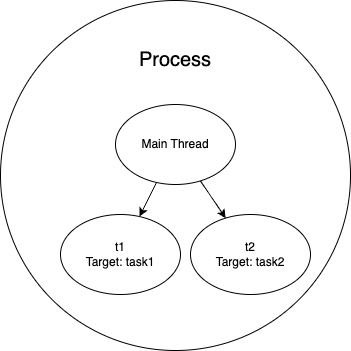
\includegraphics[width=0.5\textwidth]{D:/College/Season 3/Sistem Operasi/MID/os_report_mid2024/a_class/asset/example.png}  % Sesuaikan nama file dan ukurannya
    \caption{Ini adalah gambar contoh dari multithreading.}
    \label{fig:contoh_gambar}
\end{figure}

Seperti yang terlihat pada Gambar \ref{fig:contoh_gambar}, inilah cara menambahkan gambar dengan keterangan.

\subsection{File Systems}
File systems provide a way for the operating system to store, retrieve, and manage data. This section explains:
\begin{itemize}
    \item File system structure
    \item File access methods
    \item Directory management
\end{itemize}

\subsection{Input and Output Management}
Input and output management is key for handling the interaction between the system and external devices. This section includes:
\begin{itemize}
    \item Device drivers
    \item I/O scheduling
\end{itemize}

\subsection{Deadlock Introduction and Prevention}
Explores the concept of deadlocks and methods for preventing them:
\begin{itemize}
    \item Deadlock conditions
    \item Deadlock prevention techniques
\end{itemize}

\subsection{User Interface Management}
This section discusses the role of the operating system in managing the user interface. Topics covered include:
\begin{itemize}
    \item Graphical User Interface (GUI)
    \item Command-Line Interface (CLI)
    \item Interaction between the user and the operating system
\end{itemize}

\subsection{Virtualization in Operating Systems}
Virtualization allows multiple operating systems to run concurrently on a single physical machine. This section explores:
\begin{itemize}
    \item Concept of virtualization
    \item Hypervisors and their types
    \item Benefits of virtualization in modern computing
\end{itemize}

\section{Assignments and Practical Work}
\subsection{Assignment 1: Process Scheduling}
Students were tasked with implementing various process scheduling algorithms (e.g., FCFS, SJN, and RR) and comparing their performance under different conditions.
\subsubsection{Group 1}
\begin{python}
    class Process:
    def __init__(self, pid, arrival_time, burst_time):
        self.pid = pid
        self.arrival_time = arrival_time
        self.burst_time = burst_time
        self.completion_time = 0
        self.turnaround_time = 0
        self.waiting_time = 0
\end{python}

\begin{table}[htbp] % Optional: For floating position
    \centering
    \begin{tabular}{|c|c|c|} % Defines number of columns and alignment (c = center, l = left, r = right). '|' creates vertical lines.
    \hline
    Header 1 & Header 2 & Header 3 \\ % Column headers
    \hline
    Row 1, Column 1 & Row 1, Column 2 & Row 1, Column 3 \\ % First row of data
    \hline
    Row 2, Column 1 & Row 2, Column 2 & Row 2, Column 3 \\ % Second row of data
    \hline
    \end{tabular}
    \caption{Your table caption} % Optional: For adding a caption
    \label{tab:your_label} % Optional: For cross-referencing the table
\end{table}
\subsection{Assignment 2: Deadlock Handling}
In this assignment, students were asked to simulate different deadlock scenarios and explore various prevention methods.

\subsection{Assignment 3: Multithreading and Amdahl's Law}
This assignment involved designing a multithreading scenario to solve a computationally intensive problem. Students then applied **Amdahl's Law** to calculate the theoretical speedup of the program as the number of threads increased.

\subsection{Assignment 4: Simple Command-Line Interface (CLI) for User Interface Management}
Students were tasked with creating a simple **CLI** for user interface management. The CLI should support basic commands such as file manipulation (creating, listing, and deleting files), process management, and system status reporting.

\subsection{Assignment 5: File System Access}
In this assignment, students implemented file system access routines, including:
\begin{itemize}
    \item File creation and deletion
    \item Reading from and writing to files
    \item Navigating directories and managing file permissions
\end{itemize}

\section{Conclusion}
The first half of the course introduced core operating system concepts, including process management, scheduling, multithreading, and file system access. These topics provided a foundation for more advanced topics to be covered in the second half of the course.

\begin{thebibliography}{3}
    \bibitem{IDCloudHost}
    IDCloudHost. (n.d.). \textit{Apa Itu Software? Kenali Ciri-ciri dan Jenisnya!}. IDCloudHost. Diakses pada 3 Oktober 2024, dari https://idcloudhost.com/blog/pengertian-software-fungsi-jenis-spesifikasi-dan-contoh-software/

    \bibitem{JagoanHosting}
    Jagoan Hosting. (n.d.). \textit{Software adalah: Fungsi, jenis, dan contohnya}. JagoanHosting. Diakses pada 3 Oktober 2024, dari https://www.jagoanhosting.com/blog/software-adalah/apa-itu-software

    \bibitem{Gramedia}
    Gramedia. (n.d.). \textit{Pengertian software: Fungsi, jenis, dan contohnya}. Gramedia. Diakses pada 3 Oktober 2024, dari https://www.gramedia.com/literasi/pengetian-software/google\_vignette
\end{thebibliography}
\end{document}